\section{Kalibrasyon Metodları}
Kalibrasyon, modelin çıktılarını gerçek olasılıklara daha yakın hale getirmeyi amaçlar.
\begin{enumerate}
    \item Platt Scaling (Sigmoid Fitting)
    \item Isotonic Regression
    \item Beta Calibration
    \item Platt's Method Extension
    \item Venn-ABERS Method
\end{enumerate}

\begin{figure}[h]
    \centering
    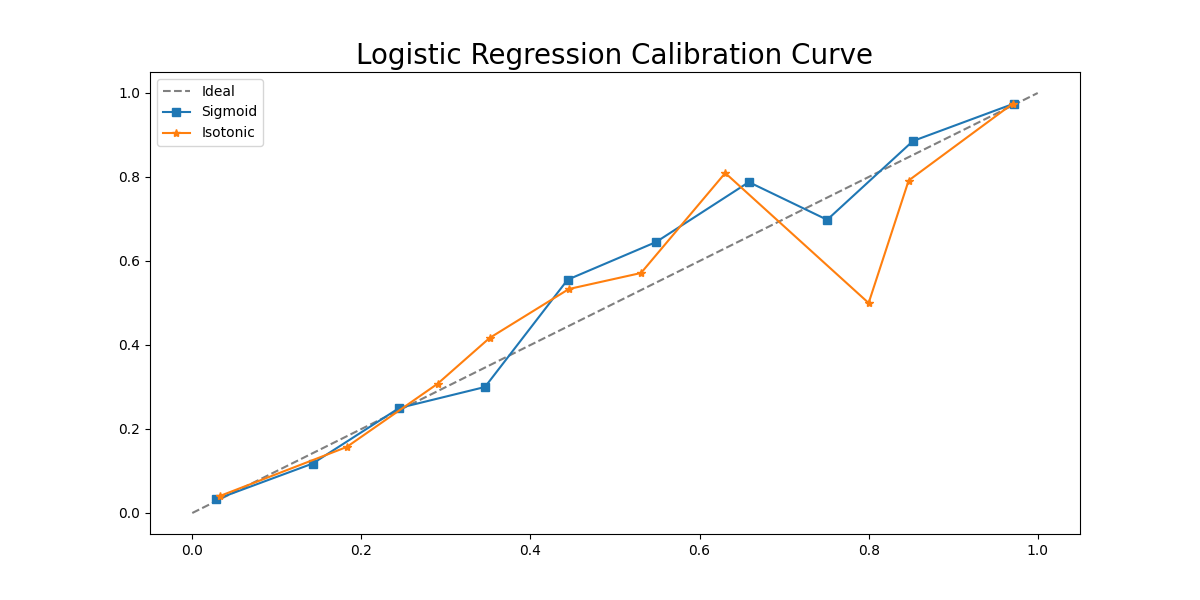
\includegraphics[width=1\textwidth]{images/calibration.png}
    \caption{Isotonic-Sigmoid kalibrasyon metodları.}
    \label{fig:enter-label}
\end{figure}

\subsection{Platt Scaling (Sigmoid Fitting)}
Adını John Platt'ten alır. Genellikle sigmoid fonksiyonu ile gerçekleştirilir. İlk olarak sınıflandırıcı çıktıları log-odds'a dönüştürülür. Ardından, log-odds değerleri sigmoid fonksiyonuna geçirilir. Bu olasılıkları [0, 1] aralığına yeniden ölçekler. Temel fikir modelin tahmin edilen sınıf olasılıklarına bir lojistik regresyon modeli uydurmaktır. Lojistik regresyon modeli, tahmin edilen olasılıklara dayalı olarak gerçek sınıf etiketlerini tahmin etmek üzere eğitilir ve modelin katsayıları tahmin edilen olasılıkları kalibre edilmiş olasılıklara dönüştürmek için kullanılır.

\[\text{platt\_cal} = \frac{1}{(1 + \exp(-z))}\]
\[\text{z} = \log(\frac{p}{1 - p})\]

\begin{lstlisting}[language=Python, caption=Scikit-learn'de Platt scaling örneği.]
from sklearn.calibration import CalibratedClassifierCV

svm = SVC(probability=True, random_state=42)
svm.fit(X_train, y_train)

calibrated_svm = CalibratedClassifierCV(svm, method='sigmoid', cv='prefit')
calibrated_svm.fit(X_train, y_train)

probabilities_before = svm.predict_proba(X_test)[:, 1]
probabilities_after = calibrated_svm.predict_proba(X_test)[:, 1]
\end{lstlisting}

\subsection{Isotonic Regression}
Olasılık tahminlerini düzgünleştirmek için monoton artan bir fonksiyonla uyumlu hale getirir. İlk olarak, modelin olasılık tahminleri sıralanır. Monoton artan bir fonksiyon olan isotonic regression kullanılır. Bu regresyon, sıralı tahminler arasında bir düzgünleştirme yaparak olasılık tahminlerini yeniden ölçekler. İzotonik, olasılıkların sırasını korur.

\begin{lstlisting}[language=Python, caption=Scikit-learn'de Isotonic Regression örneği.]
from sklearn.calibration import CalibratedClassifierCV
from sklearn.isotonic import IsotonicRegression

svm = SVC(probability=True, random_state=42)
svm.fit(X_train, y_train)

calibrated_svm = CalibratedClassifierCV(svm, method='sigmoid', cv='prefit')
calibrated_svm.fit(X_train, y_train)

probabilities_after = calibrated_svm.predict_proba(X_test)[:, 1]

isotonic_regressor = IsotonicRegression(out_of_bounds='clip')
isotonic_regressor.fit(probabilities_after, y_test)

probabilities_isotonic = isotonic_regressor.transform(probabilities_after)
\end{lstlisting}

\subsection{Beta Calibration}
Olasılık tahminlerini uygun bir şekilde düzgünleştirmek için beta dağılımını kullanır. İlk olarak, modelin olasılık tahminleri log-odds'a dönüştürülür. Ardından log-odds değerleri beta dağılımına uydurulur. Beta dağılımı [0, 1] aralığındaki değerleri modellere uygulayarak olasılık tahminlerini yeniden ölçekler.

\begin{lstlisting}[language=Python, caption=Scikit-learn'de Beta Calibration örneği.]
from sklearn.calibration import CalibratedClassifierCV
from sklearn.calibration import calibration_curve

svm = SVC(probability=True, random_state=42)
svm.fit(X_train, y_train)

calibrated_svm = CalibratedClassifierCV(svm, method='sigmoid', cv='prefit')
calibrated_svm.fit(X_train, y_train)

probabilities_after = calibrated_svm.predict_proba(X_test)[:, 1]

def beta_calibration(probabilities):
    sorted_probs = np.sort(probabilities)
    beta_values = np.linspace(0.5, len(sorted_probs) - 0.5, len(sorted_probs)) / len(sorted_probs)
    calibrated_probs = np.clip(np.interp(probabilities, sorted_probs, beta_values), 0, 1)
    return calibrated_probs

probabilities_beta = beta_calibration(probabilities_after)
\end{lstlisting}

\subsection{Platt's Method Extension}
Sigmoid dönüşümü yerine, daha genel bir logit dönüşümünü kullanır. İlk olarak modelin olasılık tahminleri logit dönüşümüne tabi tutulur. Elde edilen değerler üzerinde doğrusal bir regresyon modeli kurulur. Bu model, olasılık tahminlerini ölçeklemek için kullanılır.

\begin{lstlisting}[language=Python, caption=Scikit-learn'de Platt's Method örneği.]
from sklearn.calibration import CalibratedClassifierCV

svm = SVC(probability=True, random_state=42)
svm.fit(X_train, y_train)

calibrated_svm = CalibratedClassifierCV(svm, method='sigmoid', cv='prefit')
calibrated_svm.fit(X_train, y_train)

logit_transformed_probs = calibrated_svm.predict_proba(X_test)[:, 1] 

lr = LogisticRegression()
lr.fit(logit_transformed_probs.reshape(-1, 1), y_test)

scaled_probs = lr.predict_proba(logit_transformed_probs.reshape(-1, 1))[:, 1]
\end{lstlisting}

\subsection{Venn-ABERS}
Modelin tahminleri, modelin tahmin ettiği sınıfların gerçekte hangi oranda gerçekleştiğini gösteren bir referans dağılım ile karşılaştırılır. Karşılaştırma sonucunda, modelin tahminlerinin gerçek tahminlerden ne kadar saptığı hesaplanır. Bu sapmalar modelin tahminlerini düzeltmek için kullanılır. Dengesiz veri setlerinde etkilidir.

\begin{lstlisting}[language=Python, caption=venn\_abers kütüphanesi ile örnek.]
from venn_abers import VennAbersCalibrator
from xgboost import XGBClassifier
xgb = XGBClassifier().fit(X_train, y_train)
p_test = xgb.predict_proba(X_test)
p_cal = xgb.predict_proba(X_calib)
vac = VennAbersCalibrator()
# Inductive
ivap = vac.predict_proba(p_cal=p_cal, y_cal=y_calib, p_test=p_test)[:, 1]
# Cross
vac_c = VennAbersCalibrator(estimator=xgb, inductive=False, n_splits=10).fit(X_train, y_train)
cvap = vac_c.predict_proba(X_test)[:, 1]
\end{lstlisting}

\subsection{Metrikler}
\begin{itemize}
    \item \textbf{Brier Score:} Gerçek sınıf etiketleri ile tahmin edilen olasılıklar arasındaki farkların karesinin ortalamasıdır. Düşük brier skoru, daha iyi kalibre edilmiş bir modeli gösterir.
    \begin{equation*}
    \text{Brier Skoru} = \frac{1}{N} \sum_{i=1}^{N} (f_i - o_i)^2
    \end{equation*}
    
    Burada:
    \begin{itemize}
        \item $f_i$, $i$'inci örneğin tahmin edilen olasılığı,
        \item $o_i$, $i$'inci örneğin gerçek olasılığıdır.
    \end{itemize}
    \item \textbf{Reliability Diagram:} Gerçek sınıf olasılıkları ve modelin tahmin ettiği olasılıklar arasındaki ilişkiyi gösterir.
    \item \textbf{Calibration Curve:} Gerçek ve tahmin edilen olasılıklar arasındaki ilişkiyi görselleştiren bir eğridir. İdeal olarak eğri doğrusal olmalıdır.
\end{itemize}

\newpage